\newpage
\chapter{Results Analysis and Performance Analysis}

In our project we implemented a personalization system in which user will browse the content according to their requirement then from the searched information they will provide feedback for the relevance of that where the data will be processed through various stages as editorial planning, content reusing ,navigation and content hierarchy, Users flow and calls to action, content structure Taxonomy and Metadata ,Content development and production .This will result in the customized data to the user.

\section{Challenges Overcomed:}

1. At first it was truly hard to pick what sort of savvy part to plan. I have no involvement
with this kind of use at all and contemplating improvements without having a demo to test
on is simply so troublesome.\\
2. During the execution part, we invested a great deal of energy in finding out about Python
libraries and develops that we did not have the foggiest idea yet, similar to strings, how to
execute or do web scratching to get the connections out of a HTML page. Something else
that I needed to gain without any preparation was the means by which to make a GUI in
Python.\\
3. Something irritating was the way that I needed to creep 10000 pages more than once,
since I found in the pages different and wrong organizations. In the end the whole rundown
of organizations that I needed to boycott had a size of 18 and it included .docx,.doc,.avi,.mp4 etc.



\begin{figure}[h!]
    \begin{center}
        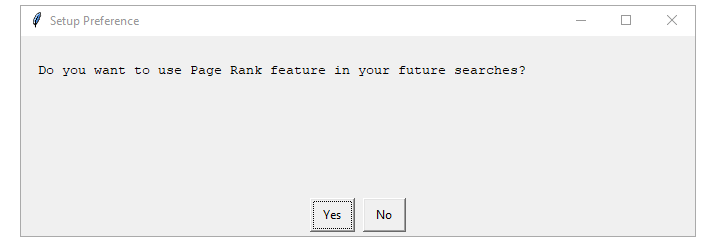
\includegraphics[scale=0.8]{res1}
        \caption{Selection for Page Rank Feature}
    \end{center}
\end{figure}
\begin{figure}[h!]
    \begin{center}
        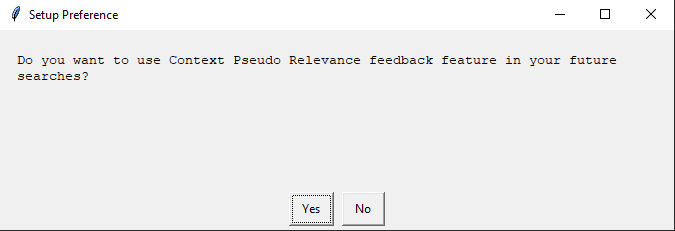
\includegraphics[scale=0.8]{res2}
        \caption{Selection for Pseudo Relevance Feedback Feature}
    \end{center}
\end{figure}

\begin{figure}[h!]
    \begin{center}
        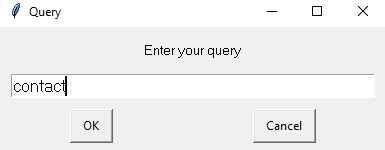
\includegraphics[scale=1]{res4}
        \caption{Input the User Query}
    \end{center}
\end{figure}
\begin{figure}[h!]
    \begin{center}
        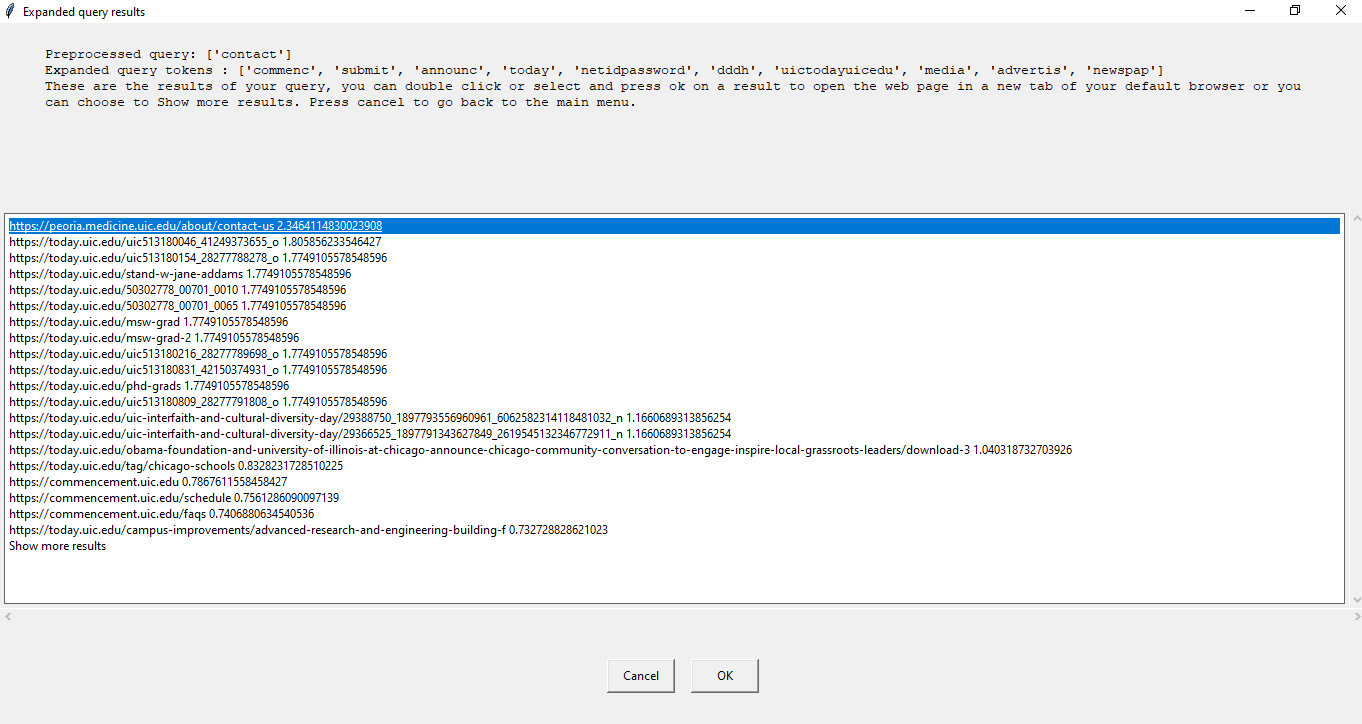
\includegraphics[scale=0.4]{res5}
        \caption{Screenshots of Project Output with generated URLs}
    \end{center}
\end{figure}
\begin{figure}[h!]
    \begin{center}
        
\includegraphics[scale=0.4]{res6}
        \caption{Screenshots of Project Output displaying generated URL}
    \end{center}
\end{figure}

\vspace{10mm}
\hrule
